\documentclass[../main.tex]{subfiles}
\graphicspath{{\subfix{images/}}}

\begin{document}

Dans cette section, vous allez expliquer les différents algorithmes qui vous paraissent importants pour votre projet. (Pour l'explication : son principe, les grandes lignes de comment il s'exécute, sa complexité,...)

\subsection{Programmation orientee objet}
Chaque élément de base du jeu est représenté par une classe. Player représente un joueur controllé par l'utilisateur, World représente le monde contenant le joueur et la map dans laquel il évolue, MatrixCase représente une case de la map, Cell représente tous les différents types de cellules et enfin Level représente un niveau de jeu.\\
Ces différentes classe sont organisées selon la hiérarchie suivante :\\

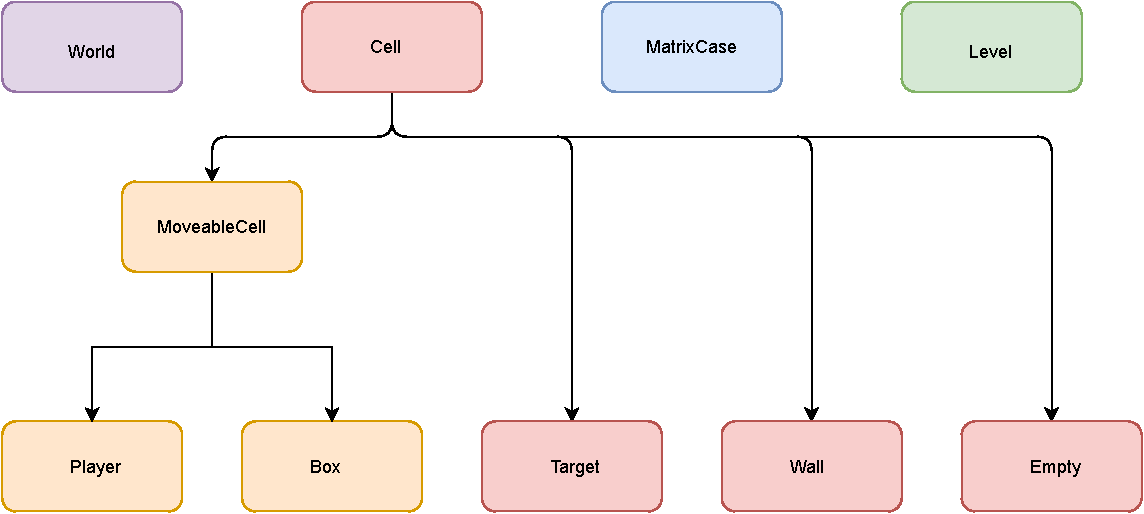
\includegraphics[width=1\textwidth,clip]{images/objects.pdf}

\subsection{Representation d'une map}
Le jeu sokoban nécessite l'implémentation de différentes cellules comme le sol, les murs, les boites, etc.. \\
Une map doit donc pouvoir contenir toutes ces cellules et permettre de les déplacer. Dans ce but, nous avons choisit de représenter une map
par une matrice. Chaque ``case'' de cette matrice est un objet instancié à partir de la classe MatrixCase. Une map est donc une matrice d'objets MatrixCase.\\
Qu'est-ce qu'une MatrixCase ? C'est un objet qui contient deux cellules. En effet une map de sokoban doit permettre la superposition de deux cellules car le joueur ou une boite peuvent se positionner au dessus du sol ou d'une cellule cible.
Schéma d'une MatrixCase :\\

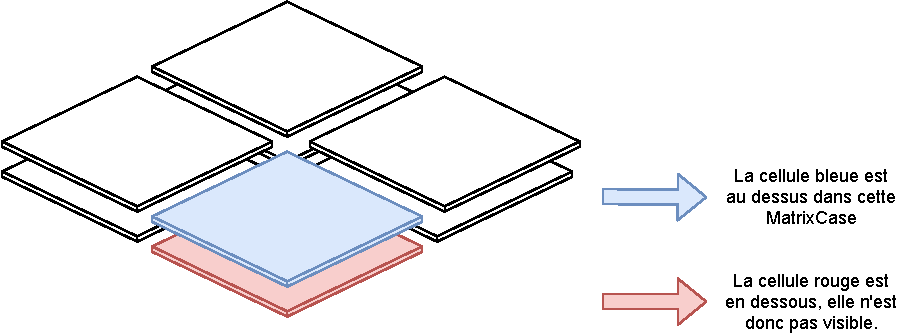
\includegraphics[width=1\textwidth,clip]{images/matrixCase.pdf}

Grâce à cette représentation d'une map, on peut accéder à n'importe quelle cellule de la matrice grâce à ses coordonnées.

\subsection{Chargement d'un niveau}

\subsection{Déplacements}

\subsection{Options utilisateur}

\subsection{Pack de textures}

\subsection{Génération aléatoire de niveau}
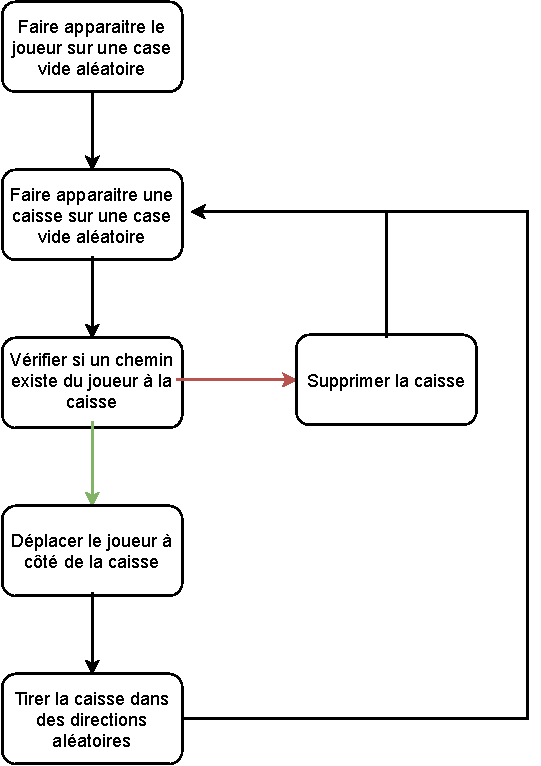
\includegraphics[width=1\textwidth]{images/generation.pdf}
\subsubsection{Placement aléatoire}
\subsubsection{Backward induction}
\subsubsection{A* path finding}

\end{document}
